% Spring Mass system in TikZ: Short Drawing Guide (Draft Version)
% Latexdraw.com
% 26/04/2021, 16:45

\documentclass[border=0.2cm]{standalone}

% Required package and libraries
\usepackage{tikz}
\usetikzlibrary{decorations.pathmorphing,patterns}

\begin{document}
	
	
	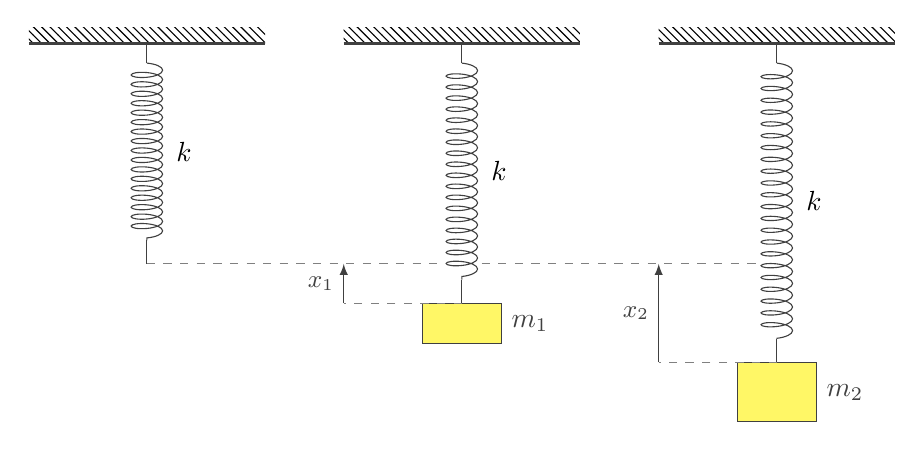
\begin{tikzpicture}[black!75]
		
		% Supporting structure
		\fill [pattern = north west lines] (-1.5,0) rectangle ++(3,.2);
		\draw[thick] (-1.5,0) -- ++(3,0);
		
		% Spring + Arrows
		\draw[] (0,0) -- ++(0,-0.25);
		\draw[decoration={aspect=0.3, segment length=1.2mm, amplitude=2mm,coil},decorate] (0,-0.25) -- ++(0,-2.25) node[midway,right=0.25cm,black]{$k$}; 
		\draw[] (0,-2.5) -- ++(0,-0.3) node[coordinate](c1){};
		
		\begin{scope}[xshift=4cm]
			% Supporting structure
			\fill [pattern = north west lines] (-1.5,0) rectangle ++(3,.2);
			\draw[thick] (-1.5,0) -- ++(3,0);
			
			% Spring + Arrows
			\draw[] (0,0) -- ++(0,-0.25);
			\draw[decoration={aspect=0.3, segment length=1.4mm, amplitude=2mm,coil},decorate] (0,-0.25) -- ++(0,-2.75) node[midway,right=0.25cm,black]{$k$}; 
			\draw[] (0,-3) -- ++(0,-0.3)node[coordinate](c2){} node[draw,fill=yellow!60,minimum width=1cm,minimum height=0.5cm,anchor=north,label=east:$m_1$](M){};
		\end{scope}
		
		\begin{scope}[xshift=8cm]
			% Supporting structure
			\fill [pattern = north west lines] (-1.5,0) rectangle ++(3,.2);
			\draw[thick] (-1.5,0) -- ++(3,0);
			
			% Spring + Arrows
			\draw[] (0,0) -- ++(0,-0.25);
			\draw[decoration={aspect=0.3, segment length=1.5mm, amplitude=2mm,coil},decorate] (0,-0.25) -- ++(0,-3.5) node[midway,right=0.25cm,black]{$k$}; 
			\draw[] (0,-3.75) -- ++(0,-0.3)node[coordinate](c3){} node[draw,fill=yellow!60,minimum width=1cm,minimum height=0.75cm,anchor=north,label=east:$m_2$](M){};
		\end{scope}
		
		
		\draw[dashed,gray] (c1) -- ++(3.75,0)coordinate(c22);
		\draw[dashed,gray] (c2) -- ++(-1.5,0) coordinate(c12);
		\draw[-latex] (c12)-- (c12|-c1)node[midway,left]{\small $x_1$};
		
		\draw[dashed,gray] (c22)++(0.5,0) -- ++(3.5,0)coordinate(c33);
		\draw[dashed,gray] (c3) -- ++(-1.5,0) coordinate(c23);
		\draw[-latex] (c23)-- (c23|-c1)node[midway,left]{\small $x_2$};
		
		
	\end{tikzpicture}
\end{document}

